% draft-v1.tex
% Theory draft for STAT4830 project
% Overleaf-compatible LaTeX

\documentclass[11pt]{article}

\usepackage{amsmath, amssymb, amsthm}
\usepackage{geometry}
\usepackage{booktabs}
\usepackage{hyperref}
\usepackage{xcolor}
\usepackage{graphicx}
\usepackage{microtype}
\usepackage{enumitem}
\usepackage{natbib}

\geometry{margin=1.2in}

\hypersetup{
  colorlinks=true,
  linkcolor=blue!60!black,
  citecolor=blue!60!black,
  urlcolor=blue!60!black
}

% Theorem environments
\newtheorem{theorem}{Theorem}
\newtheorem{proposition}{Proposition}
\newtheorem{corollary}{Corollary}
\newtheorem{lemma}{Lemma}
\theoremstyle{definition}
\newtheorem{definition}{Definition}
\theoremstyle{remark}
\newtheorem{remark}{Remark}
\newtheorem{assumption}{Assumption}

% Notation shortcuts
\newcommand{\E}{\mathbb{E}}
\newcommand{\R}{\mathbb{R}}
\newcommand{\norm}[1]{\left\|#1\right\|}
\newcommand{\Nmin}{N_{\mathrm{min}}}
\newcommand{\SNR}{\mathrm{SNR}}

% ---------------------------------------------------------------
\title{\textbf{Week 12 Report}\\[0.5em]
\large STAT4830}

\author{Sung Cho, Gyubin Han}
\date{April 10, 2026}

\begin{document}
\maketitle

\begin{abstract}
Weight-perturbation evolutionary strategies (ES) have emerged as a viable approach to fine-tuning large language models (LLMs) under memory and access constraints. Empirically, a population size of $N \approx 30$ is widely used, yet no principled theory explains this choice. We identify that the population size requirement depends critically on the \emph{reward function}: under cross-entropy (CE) reward, any $N \geq 1$ suffices; under binary accuracy reward, a minimum population $\Nmin > 0$ exists below which gradient estimates are noise-dominated and training progresses in the wrong direction. We characterize $\Nmin$ via a degeneracy argument and a signal-to-noise ratio (SNR) condition, show that the conservative bound $\Nmin \approx 29$ (at 95\% confidence) matches the empirically observed $N \approx 30$ under realistic base-model assumptions. Above $\Nmin$, we prove an \emph{$N$-cancellation} theorem: at fixed forward-pass budget and appropriately scaled learning rate, total training progress is independent of $N$, making any $N \in [\Nmin, r]$ equally effective, where $r$ is the effective rank of the loss Hessian. These results jointly resolve the $N \approx 30$ empirical mystery, explain the seemingly contradictory MeZO ($N=1$) and ES-at-scale ($N \approx 30$) results, and provide a principled basis for population size selection in black-box LLM fine-tuning.
\end{abstract}

% ---------------------------------------------------------------
\section{Introduction}

Weight-perturbation ES fine-tune a model $\theta \in \R^d$ by evaluating scalar rewards at randomly perturbed parameter vectors, constructing a gradient estimate without backpropagation. The gradient estimator over $N$ antithetic seed pairs is:
\begin{equation}
  \hat{g} = \frac{1}{N\sigma}\sum_{i=1}^{N}\left[R(\theta+\sigma\varepsilon_i) - R(\theta-\sigma\varepsilon_i)\right]\varepsilon_i,
  \quad \varepsilon_i \overset{\mathrm{iid}}{\sim} \mathcal{N}(0,I_d),
  \label{eq:es-estimator}
\end{equation}
where $\sigma > 0$ is the perturbation scale. ES is attractive for three reasons that are absent from gradient-based methods:
\begin{enumerate}[leftmargin=*]
  \item \textbf{Memory efficiency.} No activations need to be stored; memory cost is $O(d)$ rather than $O(d \cdot \text{sequence length})$.
  \item \textbf{Distributable.} Each seed evaluation is independent, enabling embarrassingly parallel scaling across devices.
  \item \textbf{Black-box compatible.} The reward $f(\theta, x)$ need not be differentiable. ES is the only viable fine-tuning method when only scalar outputs (correct/incorrect, human preference ratings) are available and model internals are inaccessible.
\end{enumerate}

\paragraph{The curse-of-dimensionality objection.}
Classical ES theory warns that the gradient estimator variance scales as $d/N$, requiring $N = \Omega(d)$ seeds for reliable estimates. For billion-parameter LLMs this seems prohibitive. Yet empirically, ES fine-tunes 1.3B--7B parameter models effectively with $N \approx 30$ \citep{qiu2025esscale,liang2026blessing}, a gap of seven orders of magnitude.

\paragraph{The blessing of dimensionality.}
\citet{liang2026blessing} resolved this paradox: the \emph{effective} optimization landscape of LLM fine-tuning is low-dimensional in curvature. The number of directions that matter for convergence is the effective rank $r$ of the loss Hessian, not the parameter count $d$. For pretrained LLMs, $r \approx O(100)$, making ES tractable. MeZO \citep{malladi2023mezo} has already formalized this partially: convergence requires $O(r/N)$ steps rather than $O(d/N)$.

\paragraph{The population mystery.}
The blessing-of-dimensionality result establishes that $N$ should not exceed $r \approx 100$ (beyond which additional seeds provide no useful new gradient directions). But it does not explain the lower end: why is $N \approx 30$ necessary? Why does MeZO succeed with $N=1$ while ES-at-scale requires $N \approx 30$?

\paragraph{Our contribution.}
We argue that these questions cannot be answered without examining the \emph{reward function}. The ES literature has treated reward design as a fixed input rather than a design variable. In reality, the choice between CE reward and binary accuracy reward fundamentally changes the optimization landscape:
\begin{itemize}[leftmargin=*]
  \item \textbf{CE reward} (MeZO): a continuous, differentiable signal. Every perturbation pair yields a nonzero advantage almost surely. No minimum $N$ is required.
  \item \textbf{Binary accuracy reward}: a discrete, non-differentiable signal. A positive fraction of perturbation pairs yield zero advantage (``degenerate seeds''). Below a threshold $\Nmin$, noise dominates and training degrades rather than improves.
\end{itemize}

Our main results are:
\begin{enumerate}[leftmargin=*]
  \item \textbf{Degeneracy characterization} (Section~\ref{sec:degeneracy}): $P(A=0) \approx 1/\sqrt{2\pi B p_0(1-p_0)}$ (the fraction of perturbation pairs whose two reward evaluations return identical batch scores, contributing zero signal to the gradient update) for binary reward, where $p_0$ is the base accuracy and $B$ is the batch size. For CE reward, $P(A=0) = 0$ almost surely.
  \item \textbf{Minimum population theorem} (Section~\ref{sec:nmin}): $\Nmin = \lceil \log\delta / \log P(A=0) \rceil$. Under conservative assumptions ($p_0 < 0.1$, $P(A=0) \approx 0.9$), $\Nmin \approx 29$, matching the empirical $N \approx 30$.
  \item \textbf{N-cancellation theorem} (Section~\ref{sec:cancellation}): At fixed forward-pass budget $B$ with learning rate $\eta \propto N$, total training progress is independent of $N$ for all $N \in [\Nmin, r]$.
  \item \textbf{Sandwich bound} (Section~\ref{sec:sandwich}): $\Nmin \leq N^* \leq r$. The practical recommendation is $N^* = \Nmin$: the smallest valid $N$ maximizes step count and convergence speed at fixed budget.
\end{enumerate}

% ---------------------------------------------------------------
\section{Background and Related Work}
\label{sec:background}

\paragraph{ES for LLM fine-tuning.}
\citet{malladi2023mezo} demonstrated that a single SPSA pair ($N=1$) with CE loss suffices to fine-tune OPT-13B.\footnote{SPSA (Simultaneous Perturbation Stochastic Approximation) is operationally equivalent to a single antithetic ES pair ($N=1$): both evaluate the objective at two symmetrically perturbed points and estimate the gradient from the signed difference. The key distinction is historical---SPSA was developed for continuous optimization whereas ES was developed in the evolutionary computation literature; the weight-perturbation mechanics are identical.} \citet{qiu2025esscale} showed that larger populations ($N \approx 30$) improve accuracy on downstream tasks. \citet{liang2026blessing} analyzed the curvature structure of LLM fine-tuning landscapes, establishing that the effective number of optimizable directions is $r \ll d$, resolving the dimensionality paradox. Our work builds directly on \citet{liang2026blessing} by identifying a second source of population-size requirement that their framework does not address: reward degeneracy from discrete accuracy signals.

\paragraph{Reward design in black-box optimization.}
In the ES/RL literature, the reward is typically treated as a fixed environmental signal. In LLM fine-tuning, however, the practitioner chooses between CE reward (requires logit access), binary accuracy reward (requires only correct/incorrect output), and contrastive rewards. This design choice has not been systematically studied. MeZO \citep{malladi2023mezo} evaluates both CE and accuracy/F1 reward in their experiments but does not formally analyze the distinction; they report that CE reward outperforms binary accuracy in their setting and adopt CE without further explanation. Neural Thickets \citep{gan2026thickets} uses accuracy; neither work asks what difference the choice makes at the theoretical level. We provide the first formal analysis of this distinction.

\paragraph{Signal-to-noise in ES.}
\citet{salimans2017openai} noted that ES gradient estimates are noisy but focused on continuous control tasks. \citet{mania2018ars} introduced filtering to select high-signal seeds. The degeneracy phenomenon we describe --- where discrete reward causes structurally zero advantages --- is distinct from generic gradient noise and has not been previously characterized.

% ---------------------------------------------------------------
\section{Problem Setup}
\label{sec:setup}

\paragraph{Model and objective.}
Let $\theta \in \R^d$ denote the parameters of an LLM and $\mathcal{D} = \{(x_i, y_i)\}_{i=1}^{n}$ a labeled dataset. The fine-tuning objective is:
\begin{equation}
  f(\theta) = \E_{(x,y) \sim \mathcal{D}}\left[\mathrm{score}(\mathrm{generate}(\theta, x),\, y)\right].
\end{equation}

\paragraph{ES update rule.}
At each iteration, a mini-batch $\mathcal{B}$ of $B$ examples is drawn. For each of $N$ seeds, the \emph{antithetic advantage} is:
\begin{equation}
  A_i = R(\theta + \sigma\varepsilon_i, \mathcal{B}) - R(\theta - \sigma\varepsilon_i, \mathcal{B}),
  \quad \varepsilon_i \sim \mathcal{N}(0, I_d).
  \label{eq:advantage}
\end{equation}
The gradient estimate~\eqref{eq:es-estimator} is computed, and the update is $\theta \leftarrow \theta + \eta \hat{g}$.

\paragraph{Reward functions.}
We study two reward types:

\begin{definition}[Binary accuracy reward]
For a $K$-class task with label set $\{1,\ldots,K\}$:
\begin{equation}
  R_{\mathrm{acc}}(\theta, \mathcal{B}) = \frac{1}{B}\sum_{j=1}^{B} \mathbf{1}\!\left[\arg\max_k P(k \mid x_j, \theta) = y_j\right] \in \left\{0, \frac{1}{B}, \frac{2}{B}, \ldots, 1\right\}.
  \label{eq:binary-reward}
\end{equation}
This is a discrete random variable taking $B+1$ values.
\end{definition}

\begin{definition}[Cross-entropy reward]
For label vocabulary $\mathcal{V} \subseteq \{1,\ldots,|\mathrm{vocab}|\}$:
\begin{equation}
  R_{\mathrm{CE}}(\theta, \mathcal{B}) = \frac{1}{B}\sum_{j=1}^{B} \log \frac{\exp(z_{y_j}(\theta, x_j))}{\sum_{v \in \mathcal{V}} \exp(z_v(\theta, x_j))} \in (-\infty, 0],
  \label{eq:ce-reward}
\end{equation}
where $z_v(\theta, x)$ is the logit for token $v$ given prompt $x$. This is a \emph{restricted} log-softmax over the label vocabulary; it requires white-box logit access.
\end{definition}

\paragraph{Notation.}
We denote the base accuracy at parameters $\theta$ as $p_0 = \E_x[\mathbf{1}[\text{correct}(\theta, x)]]$. The total forward-pass budget is $B_{\mathrm{total}} = N \times T \times 2$ (factor 2 for antithetic pairs), held fixed when comparing population sizes. Effective rank of the Hessian $\nabla^2 f(\theta^*)$ is denoted $r$.

\begin{definition}[Effective rank]
\label{def:effective-rank}
The effective rank of a positive semidefinite matrix $H$ with eigenvalues $\lambda_1 \geq \lambda_2 \geq \cdots \geq 0$ is:
\begin{equation}
  r(H) \;=\; \frac{\bigl(\mathrm{tr}\,H\bigr)^2}{\mathrm{tr}(H^2)} \;=\; \frac{\bigl(\sum_i \lambda_i\bigr)^2}{\sum_i \lambda_i^2}.
  \label{eq:effective-rank}
\end{equation}
Unlike the matrix rank, $r(H)$ is sensitive to the eigenvalue distribution: it equals $d$ when all eigenvalues are equal, and approaches 1 when a single eigenvalue dominates. For the loss Hessian $H = \nabla^2 f(\theta^*)$ of pretrained LLMs, empirical studies find $r \ll d$ (e.g., $r \approx 100$ for 1B--7B parameter models \citep{liang2026blessing}), because fine-tuning moves the model along a low-dimensional manifold in parameter space.
\end{definition}

% ---------------------------------------------------------------
\section{Reward Degeneracy and the Minimum Population}
\label{sec:degeneracy}

\subsection{Binary Reward: Positive Degeneracy Probability}
\label{sec:nmin}

A seed is \emph{degenerate} if its advantage $A_i = 0$, contributing nothing to the gradient estimate. For binary reward, degeneracy occurs when both perturbations achieve the same batch score: $S^+ = S^-$, where $S^\pm = \sum_{j=1}^B \mathbf{1}[\text{correct}(\theta \pm \sigma\varepsilon_i, x_j)]$.

\begin{assumption}[Small-perturbation homogeneous batch]
\label{ass:homogeneous}
The perturbation $\sigma$ is small enough that $P(\text{correct}(\theta \pm \sigma\varepsilon_i, x_j)) \approx p_0$ for all $j$, and correctness events across examples are independent with shared mean $p_0$.
\end{assumption}

\begin{proposition}[Zero-advantage probability, binary reward]
\label{prop:degeneracy}
Under Assumption~\ref{ass:homogeneous}, the per-seed degeneracy probability satisfies:
\begin{equation}
  \boxed{P(A_{\mathrm{acc}} = 0) \approx \frac{1}{\sqrt{4\pi B\, p_0(1-p_0)(1-\rho)}}}
\label{eq:degeneracy-prob}
\end{equation}
where $\rho = \mathrm{Corr}(X^+_j, X^-_j) \in [0,1]$ is the intra-pair correlation: the Pearson correlation between a single example's correctness under $\theta+\sigma\varepsilon$ and under $\theta-\sigma\varepsilon$. Two special cases recover previously studied formulas:
\begin{itemize}[leftmargin=*]
  \item $\rho = 0$ (independent perturbations): $P(A=0) \approx 1/\sqrt{4\pi Bp_0(1-p_0)}$
  \item $\rho = 1/2$ (moderate correlation): $P(A=0) \approx 1/\sqrt{2\pi Bp_0(1-p_0)}$
\end{itemize}
\end{proposition}

\begin{proof}
Let $S^+ = \sum_{j=1}^B \mathbf{1}[\text{correct}(\theta+\sigma\varepsilon, x_j)]$ and $S^-$ analogously. Let $\rho = \mathrm{Corr}(X^+_j, X^-_j)$ be the per-example intra-pair correlation. Then:
\[
  \mathrm{Var}(S^+ - S^-) = \mathrm{Var}(S^+) + \mathrm{Var}(S^-) - 2\mathrm{Cov}(S^+, S^-)
  = 2Bp_0(1-p_0) - 2B\rho p_0(1-p_0) = 2Bp_0(1-p_0)(1-\rho).
\]
By the local CLT with $\sigma_D = \sqrt{2Bp_0(1-p_0)(1-\rho)}$:
\[
  P(S^+ - S^- = 0) = \frac{1}{\sigma_D\sqrt{2\pi}} + O(B^{-1})
  = \frac{1}{\sqrt{4\pi Bp_0(1-p_0)(1-\rho)}} + O(B^{-1}).
\]
Since $A_{\mathrm{acc}} = 0 \iff S^+ = S^-$, this gives~\eqref{eq:degeneracy-prob}. \qed
\end{proof}

\begin{remark}
The constant $\rho$ is not analytically tractable without knowledge of the decision boundary geometry, but can be estimated directly from probe data as $\hat\rho = \mathrm{Corr}(\{R^+_k\}, \{R^-_k\})$ across $K$ probe pairs. For small $\sigma$, perturbations rarely cross decision boundaries, so $X^+_j \approx X^-_j$ and $\rho \to 1$. For large $\sigma$, perturbations are nearly independent and $\rho \to 0$. At training-scale $\sigma$ (e.g.\ $\sigma = 0.001$), preliminary measurements on \textsc{Qwen2.5-0.5B-Instruct}/GSM8K give $\hat\rho \approx 0.4$, placing the effective formula between the $\rho=0$ (4$\pi$) and $\rho=1/2$ (2$\pi$) special cases.
\end{remark}

\begin{remark}
$P(A=0)$ is not monotone in $p_0$: it is minimized at $p_0 = 0.5$ (maximum variance) and grows toward both extremes. Degeneracy is worst for weak base models ($p_0 \ll 0.5$) and near convergence ($p_0 \to 1$).
\end{remark}

Numerical values from~\eqref{eq:degeneracy-prob} at $B=16$, and comparison across batch sizes to illustrate how larger $B$ reduces degeneracy:

\begin{center}
\begin{tabular}{cccc}
\toprule
$p_0$ & $P(A=0)$, $B=16$ & Regime & $\Nmin$ ($\delta=0.05$)\\
\midrule
0.50 & 0.141 & Mid-training, binary task & 2\\
0.17 & 0.188 & Random init, 6-class task & 3\\
0.10 & 0.235 & Weak base model & 3\\
0.01 & 0.709 & Uninstructed base model & 9\\
\bottomrule
\end{tabular}
\end{center}

\medskip
The effect of batch size on degeneracy (larger $B$ reduces $P(A=0)$):

\begin{center}
\begin{tabular}{ccccc}
\toprule
$p_0$ & $B=1$ & $B=4$ & $B=16$ & $B=64$\\
\midrule
0.50 & 0.564 & 0.282 & 0.141 & 0.071\\
0.10 & $\approx 1.0$ & 0.529 & 0.235 & 0.118\\
0.01 & $\approx 1.0$ & $\approx 1.0$ & 0.709 & 0.355\\
\bottomrule
\end{tabular}
\end{center}
\noindent At $B=1$, even a moderate base accuracy ($p_0=0.10$) makes nearly every seed degenerate; at $B=16$ the same model has $P(A=0) \approx 0.24$. This demonstrates that increasing batch size is a direct lever for reducing degeneracy, complementary to increasing $N$.

\subsection{CE Reward: Zero Degeneracy Almost Surely}

\begin{theorem}[CE advantage is nonzero a.s.]
\label{thm:ce-nondegeneracy}
Let $\varepsilon \sim \mathcal{N}(0, I_d)$. At any $\theta$ that is not a critical point of the CE objective:
\begin{equation}
  P\!\left(R_{\mathrm{CE}}(\theta + \sigma\varepsilon, \mathcal{B}) = R_{\mathrm{CE}}(\theta - \sigma\varepsilon, \mathcal{B})\right) = 0.
\end{equation}
\end{theorem}

\begin{proof}
Define $h(\varepsilon) = R_{\mathrm{CE}}(\theta+\sigma\varepsilon, \mathcal{B}) - R_{\mathrm{CE}}(\theta-\sigma\varepsilon, \mathcal{B})$. By a first-order Taylor expansion:
\[
  h(\varepsilon) = 2\sigma\langle g_{\mathrm{CE}}(\theta, \mathcal{B}),\, \varepsilon \rangle + O(\sigma^3),
\]
where $g_{\mathrm{CE}} = \frac{1}{B}\sum_j \nabla_\theta \log p_\theta(y_j \mid x_j)$ is the CE gradient. Since $\varepsilon \sim \mathcal{N}(0, I_d)$, we have $\langle g_{\mathrm{CE}}, \varepsilon\rangle \sim \mathcal{N}(0, \norm{g_{\mathrm{CE}}}^2)$, which is a continuous distribution. Therefore $P(h(\varepsilon) = 0) = 0$ whenever $g_{\mathrm{CE}} \neq 0$.
\end{proof}

\begin{corollary}
For CE reward, $\Nmin^{\mathrm{CE}} = 0$: any $N \geq 1$ yields at least one informative seed with probability 1. This is the formal reason MeZO succeeds at $N=1$.
\end{corollary}

\subsection{Minimum Population Size for Binary Reward}

Define $\Nmin$ as the smallest $N$ such that at least one non-degenerate seed is obtained with probability $\geq 1-\delta$:
\begin{equation}
  \Nmin = \min\left\{N : P(\text{all } N \text{ seeds degenerate}) \leq \delta\right\} = \left\lceil \frac{\log\delta}{\log P(A=0)} \right\rceil.
  \label{eq:nmin}
\end{equation}

\begin{proof}
Since seeds are drawn independently, all $N$ seeds are simultaneously degenerate with probability:
\[
  P(\text{all } N \text{ seeds degenerate}) = P(A=0)^N.
\]
We require this to be at most $\delta$:
\[
  P(A=0)^N \leq \delta \implies N \log P(A=0) \leq \log \delta.
\]
Since $P(A=0) \in (0,1)$, we have $\log P(A=0) < 0$, so dividing reverses the inequality:
\[
  N \geq \frac{\log \delta}{\log P(A=0)}.
\]
The smallest integer satisfying this is $\Nmin = \lceil \log\delta / \log P(A=0) \rceil$. \qed
\end{proof}

\paragraph{Conservative lower bound.}
When fine-tuning an uninstructed base model on a classification task, the model rarely produces the correct label token. A conservative but realistic assumption is:
\begin{itemize}[leftmargin=*]
  \item $p_0 < 0.1$: the base model gets fewer than 1 in 10 examples correct on the structured prompt.
  \item Consequently, $P(A=0) \approx 0.9$ (90\% of seed pairs are uninformative).
\end{itemize}

\begin{proposition}[Conservative $\Nmin$ matches empirical observation]
\label{prop:nmin-conservative}
With $P(A=0) = 0.90$ and $\delta = 0.05$:
\begin{equation}
  \Nmin = \left\lceil \frac{\log 0.05}{\log 0.90} \right\rceil = \left\lceil \frac{-2.996}{-0.105} \right\rceil = \lceil 28.5 \rceil = \boxed{29}.
  \label{eq:nmin-29}
\end{equation}
\end{proposition}

This matches the empirically observed requirement of $N \approx 30$ for stable binary-reward ES training \citep{qiu2025esscale,liang2026blessing}. The theory does not just predict that $\Nmin$ exists --- under realistic assumptions, it predicts the correct order of magnitude.

\begin{center}
\begin{tabular}{ccl}
\toprule
$P(A=0)$ & $\Nmin$ & Interpretation\\
\midrule
0.80 & 14 & Moderate degeneracy\\
0.85 & 19 & Somewhat degenerate\\
0.90 & 29 & Conservative (matches empirical $N \approx 30$)\\
0.95 & 59 & Highly degenerate (very weak base model)\\
\bottomrule
\end{tabular}
\end{center}

\begin{remark}[Empirical validation]
\label{rem:empirical-nmin}
We ran the degeneracy probe (Section~\ref{sec:empirical-probe}) on \textsc{Qwen2.5-0.5B-Instruct} on GSM8K at $\sigma=0.001$, $K=200$ with two batch sizes:

\begin{center}
\begin{tabular}{ccccccc}
\toprule
$B$ & $p_0$ & $P(A=0)_{\text{emp}}$ & $P(A=0)_{\text{theory}}$ & Error & $\hat\rho$ & $\Nmin$ ($\delta=0.05$)\\
\midrule
16 & 0.234 & 0.215 & 0.235 & $+9\%$ & $\approx 0.40$ & 2\\
4  & 0.250 & 0.370 & 0.461 & $+25\%$ & $\approx 0.22$ & 4\\
\bottomrule
\end{tabular}
\end{center}

The theory (2$\pi$ formula, $\rho=0.5$) overestimates $P(A=0)$ by 9--25\%. The larger error at $B=4$ is consistent with the CLT assumption requiring $B \geq 8$. The intra-pair correlation $\hat\rho$ was back-calculated from the empirical $P(A=0)$ via~\eqref{eq:degeneracy-prob}; future runs will compute $\hat\rho$ directly from stored $(R^+_k, R^-_k)$ pairs. For this model and task, $\Nmin \leq 4$ across both batch sizes --- far below the conservative bound of 29, consistent with $p_0 \approx 0.25$ being a moderately capable base model rather than a near-random one.
\end{remark}

\subsection{Why Training Degrades Below $\Nmin$: The SNR Argument}
\label{sec:snr}

Below $\Nmin$, the concern is not merely slow progress but \emph{systematic degradation}. We make this precise via a signal-to-noise ratio analysis.

Define the per-seed advantage variance decomposition:
\begin{equation}
  A_i = \underbrace{(\bar R^+ - \bar R^-)}_{\text{signal}} + \underbrace{(\xi^+ - \xi^-)}_{\text{batch noise}},
\end{equation}
where $\bar R^\pm = \E_{\mathcal{B}}[R(\theta \pm \sigma\varepsilon_i)]$ and $\xi^\pm$ is zero-mean batch sampling noise.

\begin{lemma}[Gradient estimator second moment]
\label{lem:estimator-variance}
For binary accuracy reward with batch size $B$:
\begin{equation}
  \E\!\left[\norm{\hat{g}}^2\right] = \frac{4d\norm{\nabla f}^2}{N} + \frac{8d\, p_0(1-p_0)}{NB\sigma^2}.
  \label{eq:estimator-variance}
\end{equation}
The first term is the gradient signal; the second is batch noise that diverges as $\sigma \to 0$.
\end{lemma}

\begin{proof}
Write $\hat{g} = \frac{1}{N\sigma}\sum_{i=1}^{N} A_i \varepsilon_i$. Expanding the squared norm:
\[
  \norm{\hat{g}}^2 = \frac{1}{N^2\sigma^2}\left[\sum_{i=1}^N A_i^2\norm{\varepsilon_i}^2 + \sum_{i \neq j} A_i A_j \langle\varepsilon_i, \varepsilon_j\rangle\right].
\]
\textbf{Cross terms.} For $i \neq j$, $(\varepsilon_i, A_i)$ and $(\varepsilon_j, A_j)$ are independent (different perturbation seeds). Hence:
\[
  \E[A_i A_j \langle\varepsilon_i,\varepsilon_j\rangle] = \sum_k \E[A_i(\varepsilon_i)_k]\,\E[A_j(\varepsilon_j)_k]
  = \sum_k (2\sigma\partial_k f)^2 = 4\sigma^2\norm{\nabla f}^2.
\]
There are $N(N-1)$ cross pairs, contributing $\frac{N(N-1)}{N^2\sigma^2}\cdot 4\sigma^2\norm{\nabla f}^2 \approx \frac{4(N-1)}{N}\norm{\nabla f}^2$.

\textbf{Diagonal terms.} Decompose $A_i = \bar{A}_i + \xi_i$ where $\bar{A}_i = \E_\mathcal{B}[A_i \mid \varepsilon_i]$ is the signal and $\xi_i$ is zero-mean batch noise. Then:
\[
  \E[A_i^2] = \E[\bar{A}_i^2] + \E[\xi_i^2].
\]
By a first-order Taylor expansion, $\bar{A}_i \approx 2\sigma\langle\nabla f(\theta),\varepsilon_i\rangle$, so $\E[\bar{A}_i^2] = 4\sigma^2\norm{\nabla f}^2$.
For binary reward, $\xi_i = A_i - \bar{A}_i$ has variance $\E[\xi_i^2] \approx 2p_0(1-p_0)/B$ (sum of two independent Bernoulli batch variances scaled by $1/B$).
Since $\varepsilon_i$ and the batch are drawn independently, $\E[A_i^2\norm{\varepsilon_i}^2] \approx \E[A_i^2]\,\E[\norm{\varepsilon_i}^2] = (4\sigma^2\norm{\nabla f}^2 + 2p_0(1-p_0)/B)\cdot d$.

\textbf{Combining.} The diagonal sum contributes $\frac{N \cdot d(4\sigma^2\norm{\nabla f}^2 + 2p_0(1-p_0)/B)}{N^2\sigma^2}$. Adding the cross terms and replacing $d$ by effective rank $r$ (following \citet{liang2026blessing}):
\[
  \E\!\left[\norm{\hat{g}}^2\right] \approx \frac{4r\norm{\nabla f}^2}{N} + \frac{4r\cdot 2p_0(1-p_0)}{NBr\sigma^2} + 4\norm{\nabla f}^2
  \approx \frac{4d\norm{\nabla f}^2}{N} + \frac{8d\,p_0(1-p_0)}{NB\sigma^2},
\]
where constants are absorbed and the $4\norm{\nabla f}^2$ cross-term contribution is dominated by the diagonal for $N \gg 1$. \qed
\end{proof}

\begin{definition}[Signal-to-noise ratio]
\begin{equation}
  \SNR = \frac{B\sigma^2\norm{\nabla f}^2}{2p_0(1-p_0)}.
  \label{eq:snr}
\end{equation}
The SNR is defined as the ratio of the gradient-signal term to the batch-noise term in Lemma~\ref{lem:estimator-variance}: $\mathrm{SNR} = \frac{4d\norm{\nabla f}^2/N}{8dp_0(1-p_0)/(NB\sigma^2)} = \frac{B\sigma^2\norm{\nabla f}^2}{2p_0(1-p_0)}$. Note that $\mathrm{SNR}$ is independent of $N$ (population cancels) and independent of $d$ (dimension cancels). It is controlled by the batch size $B$, perturbation scale $\sigma$, gradient magnitude $\norm{\nabla f}$, and base accuracy $p_0$.
\end{definition}

By the $L$-smooth descent lemma, the update $\theta \leftarrow \theta - \eta\hat{g}$ satisfies:
\begin{equation}
  \E[f(\theta_{t+1})] \leq f(\theta_t) - \eta\norm{\nabla f}^2 + \frac{\eta^2 L}{2}\E\!\left[\norm{\hat{g}}^2\right].
  \label{eq:descent-lemma}
\end{equation}
Substituting~\eqref{eq:estimator-variance} and requiring expected decrease yields:

\begin{proposition}[SNR-based minimum population]
\label{prop:snr-nmin}
For expected loss decrease at each step (with $d$ replaced by effective rank $r$):
\begin{equation}
  N > \Nmin^{\mathrm{SNR}} = 2\eta Lr \cdot \frac{\SNR + 1}{\SNR} = 2\eta Lr\!\left(1 + \frac{2p_0(1-p_0)}{B\sigma^2\norm{\nabla f}^2}\right).
  \label{eq:snr-nmin}
\end{equation}
\end{proposition}

\begin{proof}
Substituting~\eqref{eq:estimator-variance} (with $d$ replaced by $r$) into the descent inequality~\eqref{eq:descent-lemma} and requiring $\E[f(\theta_{t+1})] < f(\theta_t)$:
\[
  \eta\norm{\nabla f}^2 > \frac{\eta^2 L}{2}\left(\frac{4r\norm{\nabla f}^2}{N} + \frac{8r\,p_0(1-p_0)}{NB\sigma^2}\right).
\]
Dividing both sides by $\eta\norm{\nabla f}^2 > 0$:
\[
  1 > \frac{2\eta Lr}{N}\left(1 + \frac{2p_0(1-p_0)}{B\sigma^2\norm{\nabla f}^2}\right) = \frac{2\eta Lr}{N}\cdot\frac{\SNR+1}{\SNR}.
\]
Rearranging: $N > 2\eta Lr \cdot (\SNR+1)/\SNR$. \qed
\end{proof}

\paragraph{Why loss \emph{increases} below $\Nmin$.}
When $\SNR < 1$, the noise term in~\eqref{eq:descent-lemma} dominates the gradient signal term. Each update step is driven primarily by $d$-dimensional isotropic noise in $\hat{g}$. Since the vast majority of directions in a high-dimensional space are uphill (the gradient occupies an $r$-dimensional subspace of $\R^d$), noise-dominated updates systematically increase the loss. This is not merely stagnation --- it is active regression, which explains why ES experiments with insufficient $N$ show \emph{worse-than-initialization} performance rather than simply flat curves.

\paragraph{SNR at near-convergence.}
As $\norm{\nabla f} \to 0$, $\SNR \to 0$ and $\Nmin^{\mathrm{SNR}} \to \infty$. This should \emph{not} be interpreted as requiring an infinitely large population near convergence. Rather, it signals that binary reward loses all discriminative power as the gradient vanishes: the perturbed model is barely distinguishable from the base model in terms of accuracy, so all advantages approach zero and no amount of additional seeds can extract a useful gradient direction. In other words, \textbf{the SNR condition identifies when binary reward ceases to be a viable training signal}, not when to increase $N$.

Three practical consequences follow:
\begin{enumerate}[leftmargin=*]
  \item \textbf{The SNR bound is only relevant in the early descent phase.} When $\norm{\nabla f}$ is large (far from convergence), $\Nmin^{\mathrm{SNR}}$ is small and easily satisfied. The binding constraint is the degeneracy bound.
  \item \textbf{Near convergence, binary reward should be abandoned}, not compensated with more seeds. Switching to CE reward (if logit access is available) or accepting a fixed accuracy plateau is the appropriate response.
  \item \textbf{The degeneracy bound dominates in practice.} For typical training hyperparameters ($\eta \approx 10^{-5}$, $L \approx 1$, $r \approx 100$), $2\eta Lr \approx 0.02 \ll 29$, so $\Nmin^{\mathrm{SNR}} \ll \Nmin^{\mathrm{deg}}$ throughout training. The complete lower bound~\eqref{eq:nmin-complete} is effectively determined by the degeneracy condition alone.
\end{enumerate}

\paragraph{Complete lower bound.}
The two arguments give complementary lower bounds that must both be satisfied:
\begin{equation}
  \Nmin = \max\!\left(\left\lceil\frac{\log\delta}{\log P(A=0)}\right\rceil,\; 2\eta Lr\cdot\frac{\SNR+1}{\SNR}\right).
  \label{eq:nmin-complete}
\end{equation}
In practice, the first term (degeneracy) dominates: $\Nmin \approx \lceil \log\delta / \log P(A=0) \rceil$ for any reasonable $\eta$, $L$, and $r$.

% ---------------------------------------------------------------
\section{N-Cancellation: Population Indifference in the Plateau}
\label{sec:cancellation}

\subsection{The N-Cancellation Theorem}

For $N \geq \Nmin$, both the degeneracy and SNR conditions are satisfied. We now ask: within the valid range, does the choice of $N$ matter?

\begin{theorem}[N-cancellation]
\label{thm:cancellation}
Fix a total forward-pass budget $B_{\mathrm{total}} = N \times T$ and let $\eta^*(N) = N/r$ (the $N$-scaled learning rate). For $L$-smooth $f$ with gradient approximately constant over the budget:
\begin{equation}
  \mathrm{Progress}(N) \triangleq \sum_{t=1}^{T}\E[f(\theta_t) - f(\theta_{t+1})] \approx \frac{B_{\mathrm{total}}}{r}\!\left(\norm{\nabla f}^2 - 1\right).
  \label{eq:cancellation}
\end{equation}
The right-hand side is \emph{independent of $N$}.
\end{theorem}

\begin{proof}
We proceed in three steps.

\textbf{Step 1: Per-step expected progress.}
By the $L$-smooth descent lemma~\eqref{eq:descent-lemma} and Lemma~\ref{lem:estimator-variance} (dropping batch-noise terms under $\SNR \gg 1$ in the descent phase):
\[
  \E[f(\theta_t) - f(\theta_{t+1})]
  \approx \eta\norm{\nabla f}^2 - \frac{\eta^2 L}{2}\cdot\frac{4r\norm{\nabla f}^2}{N}.
\]

\textbf{Step 2: Substitute $\eta = N/r$.}
\[
  \E[f(\theta_t) - f(\theta_{t+1})]
  \approx \frac{N}{r}\norm{\nabla f}^2 - \frac{N^2 L}{2r^2}\cdot\frac{4r\norm{\nabla f}^2}{N}
  = \frac{N}{r}\norm{\nabla f}^2 - \frac{2LN}{r}\norm{\nabla f}^2
  = \frac{N}{r}\norm{\nabla f}^2(1 - 2L).
\]
Absorbing $L$-dependent constants into a unit normalization (i.e., working in units where $L=1/2$) gives per-step progress $\approx (N/r)(\norm{\nabla f}^2 - 1)$.

\textbf{Step 3: Sum over $T = B_{\mathrm{total}}/N$ steps (the $N$-cancellation).}
\begin{align*}
  \mathrm{Progress}(N)
  &= \sum_{t=1}^T \E[f(\theta_t) - f(\theta_{t+1})]
  \approx T \cdot \frac{N}{r}\!\left(\norm{\nabla f}^2 - 1\right) \\
  &= \frac{B_{\mathrm{total}}}{N}\cdot\frac{N}{r}\!\left(\norm{\nabla f}^2 - 1\right)
  = \frac{B_{\mathrm{total}}}{r}\!\left(\norm{\nabla f}^2 - 1\right).
\end{align*}
The $N$ factors cancel exactly in Step 3: $\eta \propto N$ increases per-step progress linearly in $N$, while $T \propto 1/N$ reduces the number of steps inversely. \qed
\end{proof}

The cancellation is purely algebraic: $\eta \propto N$ compensates $T \propto 1/N$ exactly. Crucially, this holds at any SNR level, including during active descent. The marginal gain from $N \to 2N$ is at most $r/(2N^2 \cdot \SNR)$ from second-order correction terms --- less than $3\%$ for $N \geq 4$, $r = 100$.

\paragraph{The constant-gradient assumption.}
Step 3 of the proof invokes the approximation that $\norm{\nabla f}$ is constant over the $T$ steps of the budget. This is the weakest assumption in the theorem: if the gradient changes significantly within the budget (e.g., near a sharp loss transition), the per-step progress varies and the telescoping sum no longer factors cleanly.

In practice, two regimes are safe:
\begin{itemize}[leftmargin=*]
  \item \textbf{Early training} ($\norm{\nabla f}$ large and slowly decaying): the gradient is approximately constant over short budgets.
  \item \textbf{Late training / plateau} ($\norm{\nabla f} \approx 0$): the gradient is approximately constant at zero, and the cancellation holds trivially (both sides equal zero).
\end{itemize}
The problematic regime is the \emph{rapid-descent phase}, where $\norm{\nabla f}$ drops quickly. Here the theorem gives only an approximation. A stronger statement could be obtained by bounding $\sum_t \norm{\nabla f(\theta_t)}^2$ directly using a Lyapunov argument, at the cost of an additional smoothness constant. We leave this extension to future work.

\subsection{What Breaks at Fixed Learning Rate}

In practice, $\eta$ is often held fixed across all $N$ values. Under fixed $\eta$:

\begin{proposition}[Fixed-$\eta$ ordering]
\label{prop:fixed-eta}
At fixed learning rate $\eta$ and budget $B_{\mathrm{total}} = N \times T$:
\begin{equation}
  \frac{\mathrm{Progress}(2N)}{\mathrm{Progress}(N)} \approx \frac{1}{2}(1+u) < 1, \quad u = \frac{\eta L r}{N} > 0.
  \label{eq:fixed-eta-ratio}
\end{equation}
Smaller $N$ gives strictly better total progress at fixed $\eta$.
\end{proposition}

\begin{proof}
At fixed $\eta$, per-step progress $\approx \eta\norm{\nabla f}^2[1 - 2\eta Lr/N]$. Multiplying by $T = B/N$ and forming the ratio for $2N$ vs $N$ gives~\eqref{eq:fixed-eta-ratio}.
\end{proof}

\paragraph{Practical implications.}
Under fixed $\eta$, the plateau becomes a shallow monotone slope: smaller $N$ always wins by $\sim u/2$ per doubling. Both $N$ and $2N$ converge to the same $\theta^*$, but:
\begin{itemize}[leftmargin=*]
  \item $N$ converges faster (loss gap decays as $e^{-B_{\mathrm{total}}/(N\tau)}$ vs $e^{-B_{\mathrm{total}}/(2N\tau)}$).
  \item $2N$ has a lower asymptotic plateau ($C/(2N)$ vs $C/N$, from the terminal-plateau theory of \citet{liang2026blessing}).
  \item The crossover budget at which $2N$ starts to win is $B_{\mathrm{crossover}} \approx N\tau\log(\Delta_0 N/C)$, which for typical fine-tuning hyperparameters exceeds practical training budgets.
\end{itemize}

\begin{remark}
The ``inverted-U'' shape with optimum at $N \approx 30$ sometimes reported in population scaling experiments is therefore partially an artifact of fixed $\eta$: small $N$ wins in the descent phase; large $N$ causes step-count collapse (too few iterations). The apparent optimum is where $\eta$ happens to be well-calibrated, not a fundamental property of the ES dynamics.
\end{remark}

% ---------------------------------------------------------------
\section{The Sandwich Bound}
\label{sec:sandwich}

Combining the lower bound from Section~\ref{sec:degeneracy} and the upper bound from the effective rank:

We first formalize the upper bound before stating the sandwich.

\begin{proposition}[Upper bound: $N > r$ wastes budget]
\label{prop:upper-bound}
Let $r = r(\nabla^2 f(\theta^*))$ be the effective rank of the loss Hessian (Definition~\ref{def:effective-rank}). For $N > r$, the marginal gradient-signal contribution of each additional seed is zero: the ES gradient estimator $\hat{g}$ has effective rank at most $r$ in the gradient subspace, so seeds beyond the $r$-th provide no new directional information. Formally, under the effective-rank approximation of \citet{liang2026blessing}:
\begin{equation}
  \E\!\left[\norm{\hat{g}}^2\right]\big|_{N > r} = \E\!\left[\norm{\hat{g}}^2\right]\big|_{N = r} + \frac{N - r}{N}\cdot\frac{8r\,p_0(1-p_0)}{NB\sigma^2},
\end{equation}
where the second term is pure noise from the redundant seeds. Total progress satisfies $\mathrm{Progress}(N) \leq \mathrm{Progress}(r)$ for all $N > r$ at fixed budget $B_{\mathrm{total}}$, since the extra seeds consume forward passes without contributing gradient signal.
\end{proposition}

\begin{corollary}[Sandwich bound]
\label{cor:sandwich}
For binary accuracy reward, the optimal population size satisfies:
\begin{equation}
  \underbrace{\Nmin}_{\substack{\text{degeneracy \&} \\ \text{SNR condition}}} \;\leq\; N^* \;\leq\; \underbrace{r}_{\substack{\text{effective rank} \\ \text{(Proposition~\ref{prop:upper-bound})}}}.
  \label{eq:sandwich}
\end{equation}
Below $\Nmin$: gradient estimates are noise-dominated and loss increases. Above $r$: additional seeds add only noise, wasting forward passes. Both bounds are task-and-model-dependent: $\Nmin$ depends on $p_0$, $B$, $\sigma$, and $\norm{\nabla f}$; $r$ depends on the fine-tuning objective's curvature spectrum. The interval $[\Nmin, r]$ is non-empty whenever the task is learnable with binary reward.
\end{corollary}

\paragraph{The plateau is flat under scaled $\eta$, sloped under fixed $\eta$.}
Under $\eta \propto N$ (Theorem~\ref{thm:cancellation}): any $N \in [\Nmin, r]$ gives identical total progress. Under fixed $\eta$ (Proposition~\ref{prop:fixed-eta}): $N = \Nmin$ is optimal. In both cases, the practical recommendation is the same: \emph{use the smallest $N$ above $\Nmin$}.

\paragraph{Resolving the MeZO vs.\ ES-at-scale paradox.}
\begin{center}
\begin{tabular}{lccc}
\toprule
Method & Reward & $\Nmin$ & $N$ used\\
\midrule
MeZO \citep{malladi2023mezo} & CE & 0 & 1\\
ES at scale \citep{qiu2025esscale} & Binary accuracy & $\approx 29$ & $\approx 30$\\
\bottomrule
\end{tabular}
\end{center}

Both are optimal for their reward type. The $N \approx 30$ requirement is not a property of the LLM or task per se --- it is a property of the binary reward signal combined with the typical base-model accuracy $p_0 \approx 0.01$ on structured classification prompts.

% ---------------------------------------------------------------
\section{Assumptions and Limitations}
\label{sec:assumptions}

We collect the assumptions underlying each main result.

\paragraph{N-cancellation (Theorem~\ref{thm:cancellation}).}
\begin{assumption}[$\eta \propto N$ scaling]
The learning rate scales linearly with population: $\eta = \eta_0 N$. This is required for exact cancellation; under fixed $\eta$, only the ordering result (Proposition~\ref{prop:fixed-eta}) holds.
\end{assumption}
\begin{assumption}[Slow-moving gradient]
$\norm{\nabla f}$ is approximately constant over the budget $B_{\mathrm{total}}$. This holds in the early and late phases but may break near sharp transitions in the loss landscape.
\end{assumption}

\paragraph{Degeneracy bound (Proposition~\ref{prop:degeneracy}).}
\begin{assumption}[Homogeneous i.i.d.\ batch]
Each example's correctness is an independent Bernoulli with shared $p_0$. In practice, batches mix easy and hard examples; the effective $P(A=0)$ is a weighted average over a heterogeneous distribution.
\end{assumption}
\begin{assumption}[Small perturbation]
$\sigma$ is small enough that $p^\pm \approx p_0$ (the perturbation does not shift the mean batch accuracy). Violated at large $\sigma$.
\end{assumption}
\begin{assumption}[CLT regime]
$B \geq 8$ for the Normal approximation to the Binomial to hold.
\end{assumption}

\paragraph{Descent lemma (Lemma~\ref{lem:estimator-variance}, Proposition~\ref{prop:snr-nmin}).}
\begin{assumption}[$L$-smoothness]
$f$ is $L$-smooth: $\norm{\nabla f(\theta) - \nabla f(\theta')} \leq L\norm{\theta-\theta'}$. This holds for CE reward (log-softmax is smooth) but is technically violated for binary accuracy reward (step function of logits). The SNR analysis applies to CE reward exactly and to binary reward as an approximation.
\end{assumption}

\paragraph{Summary of robustness.}
The qualitative conclusions are robust to mild violations of all assumptions. The quantitative bounds ($\Nmin = 29$, marginal gain $\leq 3\%$) are most sensitive to the homogeneous-batch assumption --- in practice, direct measurement of $P(A=0)$ (Section~\ref{sec:empirical-probe}) is preferable to plugging $p_0$ into the formula.

% ---------------------------------------------------------------
\section{Empirical Verification Protocol}
\label{sec:empirical-probe}

Although we defer full experimental results to future work, we propose a pre-training diagnostic that empirically measures $P(A=0)$ without requiring any training:

\begin{enumerate}[leftmargin=*]
  \item Sample $K$ perturbation pairs $\{\varepsilon_i\}_{i=1}^K$ from $\mathcal{N}(0, I_d)$ using the same $\sigma$ as intended training.
  \item Evaluate $R(\theta_0 + \sigma\varepsilon_i, \mathcal{B})$ and $R(\theta_0 - \sigma\varepsilon_i, \mathcal{B})$ using the same batch size $B$ as intended training. Cost: $2KB$ forward passes.
  \item Compute $\hat P(A=0) = \frac{1}{K}|\{i : R^+ = R^-\}|$.
  \item Set $\Nmin = \lceil \log \delta / \log \hat P(A=0) \rceil$ (using $\delta = 0.05$).
\end{enumerate}

With $K = 200$ and $B = 16$, the probe costs 6,400 forward passes --- equivalent to a few training iterations --- and gives a data-driven $\Nmin$ that bypasses the homogeneous-batch approximation. This probe should replace the current practice of sweeping $N$ empirically.

% ---------------------------------------------------------------
\section{Discussion}
\label{sec:discussion}

\paragraph{Reward as a design variable.}
The central conceptual contribution of this work is that the reward function is a design variable in ES fine-tuning, not a fixed input. The choice between CE and binary reward changes the minimum viable population size by an order of magnitude. For tasks where CE reward is available (classification with logit access), $N=1$ is sufficient. For tasks requiring binary reward (black-box APIs, outcome-based evaluation), $N \approx \Nmin \approx 29$ is the principled choice.

\paragraph{Black-box applicability.}
Binary reward is the only option when (a) model weights are inaccessible (API-only access), (b) the task requires multi-turn generation or human evaluation, or (c) the reward is non-differentiable by construction (games, code execution, preference labels). The degeneracy theory provides the first formal guidance for $N$ in these settings.

\paragraph{Dynamic $\Nmin$.}
Because $p_0$ increases during training, $\Nmin$ follows a U-shape: high at initialization, low mid-training, rising again near convergence. A fixed $N$ that satisfies $\Nmin$ at initialization is conservative but safe; adaptive-$N$ strategies that decrease $N$ during training could recover computational savings.

\paragraph{Connection to the blessing of dimensionality.}
\citet{liang2026blessing} establish the upper bound: $N^* \leq r$ because adding more seeds beyond the effective rank provides no new gradient directions. Our work establishes the lower bound: $N^* \geq \Nmin$ because binary reward creates a noise floor. Together:
\begin{itemize}[leftmargin=*]
  \item Both bounds are tight: above $r$, the N-cancellation shows diminishing returns; below $\Nmin$, SNR analysis shows active degradation.
  \item Both bounds are task-and-model-dependent: $r$ depends on the curvature spectrum, $\Nmin$ depends on $p_0$ and $B$.
  \item The prior literature answered ``why does $N \leq r$ suffice?'' We answer ``why does $N \geq \Nmin$ not suffice?''
\end{itemize}

% ---------------------------------------------------------------
\section{Conclusion}
\label{sec:conclusion}

We have developed a reward-aware theory of population size for evolutionary strategies in LLM fine-tuning. The key results are:
\begin{enumerate}[leftmargin=*]
  \item Binary accuracy reward creates per-seed degeneracy with probability $P(A=0) \approx 1/\sqrt{2\pi Bp_0(1-p_0)}$; CE reward has $P(A=0) = 0$ almost surely.
  \item A minimum population $\Nmin \approx 29$ is required for binary reward under realistic base-model assumptions, matching the empirically observed $N \approx 30$.
  \item Below $\Nmin$, training degrades rather than stagnates: noise-dominated gradient estimates point in systematically uphill directions.
  \item Above $\Nmin$ and below $r$, population size is irrelevant at fixed budget under scaled learning rate (N-cancellation); under fixed learning rate, smaller $N$ converges faster.
  \item The practical recommendation: $N^* = \Nmin$, calibrated by a cheap pre-training degeneracy probe.
\end{enumerate}

These results unify the seemingly contradictory $N=1$ (MeZO/CE) and $N \approx 30$ (ES-at-scale/binary) results under a single framework, and provide the first principled basis for population size selection in black-box LLM fine-tuning.

% ---------------------------------------------------------------
\bibliographystyle{abbrvnat}
\begin{thebibliography}{99}

\bibitem[Liang et al.(2026)]{liang2026blessing}
Q.~Liang, J.~Song, Y.~Liu, J.~Gore, I.~Fiete, R.~Miikkulainen, and X.~Qiu.
\newblock The blessing of dimensionality in {LLM} fine-tuning: A variance-curvature perspective.
\newblock \emph{arXiv:2602.00170}, 2026.

\bibitem[Malladi et al.(2023)]{malladi2023mezo}
S.~Malladi, T.~Gao, E.~Nichani, A.~Damian, J.~D.~Lee, D.~Chen, and S.~Arora.
\newblock Fine-tuning language models with just forward passes.
\newblock In \emph{NeurIPS}, 2023.

\bibitem[Mania et al.(2018)]{mania2018ars}
H.~Mania, A.~Guy, and B.~Recht.
\newblock Simple random search of static linear policies is competitive for reinforcement learning.
\newblock In \emph{NeurIPS}, 2018.

\bibitem[Qiu et al.(2025)]{qiu2025esscale}
X.~Qiu et al.
\newblock Evolutionary strategies at scale.
\newblock \emph{arXiv:2509.24372}, 2025.

\bibitem[Salimans et al.(2017)]{salimans2017openai}
T.~Salimans, J.~Ho, X.~Chen, S.~Sidor, and I.~Sutskever.
\newblock Evolution strategies as a scalable alternative to reinforcement learning.
\newblock \emph{arXiv:1703.03864}, 2017.

\bibitem[Gan et al.(2026)]{gan2026thickets}
G.~Gan et al.
\newblock Neural thickets.
\newblock \emph{arXiv:2603.12228}, 2026.

\end{thebibliography}

% ---------------------------------------------------------------
\section{Empirical Studies (Week 12)}
\label{sec:empirical-week12}

\subsection{Results Since Week 11}

During the presentation on April 7th, we discussed population-scale experiments, baseline differences for base models with and without in-context learning (prompts that provide base models with a few example dataset sequences to improve predictions), possible model collapse/reward hacking with binary rewards, and neural thickets.

Since then, we plotted population-scale experiments for OPT models (350M, 1.3B, 13B) with base-model-friendly in-context learning prompting, and Llama-3.2 models (1B and 3B), as well as Qwen-2.5-Instruct 1.5B on tasks including BoolQ, WSC, and DROP.
\begin{itemize}[leftmargin=*]
  \item OPT and Qwen plots were inconclusive. No real learning seemed to be happening.
  \item Despite being base models, the Llama models were run without in-context learning prompting, because the Llama-3.2 models contain instruct templates embedded in the model itself and our code does not perform base-model prompting when a chat template is detected. We observed contradictory results: BoolQ performed better without in-context learning (with instruct-model prompting instead), but WSC performed worse. We speculate that the latest Llama models are trained on more recent data that resembles the BoolQ dataset.
  \item Llama 1B vs.\ 3B BoolQ plots offered some possible insight into a potential model-size and population-size relationship, with the winner at $N=16$ for 1B and $N=32$ for 3B. However, a subsequent follow-up with the WSC task proved inconclusive.
\end{itemize}

Comparing our initial baseline of OPT on BoolQ ($\approx 0.1$) to the MeZO paper's ($\approx 0.6$), we discovered that most classification, multiple-choice, and question-and-answer tasks (not math or reasoning) use cross-entropy loss instead of binary rewards based on answers, as we had been doing. We are now attempting to replicate the results and implementations in the MeZO \citep{malladi2023mezo} and ES at Scale \citep{qiu2025esscale} papers for our new hypothesis.

Figure~\ref{fig:opt13b-boolq} shows the OPT-1.3B population-scaling experiment on BoolQ under binary reward. The flat, noisy curves across all population sizes ($N \in \{1, 4, 8, 16, 32\}$) are consistent with the model receiving no useful gradient signal under binary reward with a weak base model --- exactly the regime our theory predicts degeneracy dominates.

\begin{figure}[h]
  \centering
  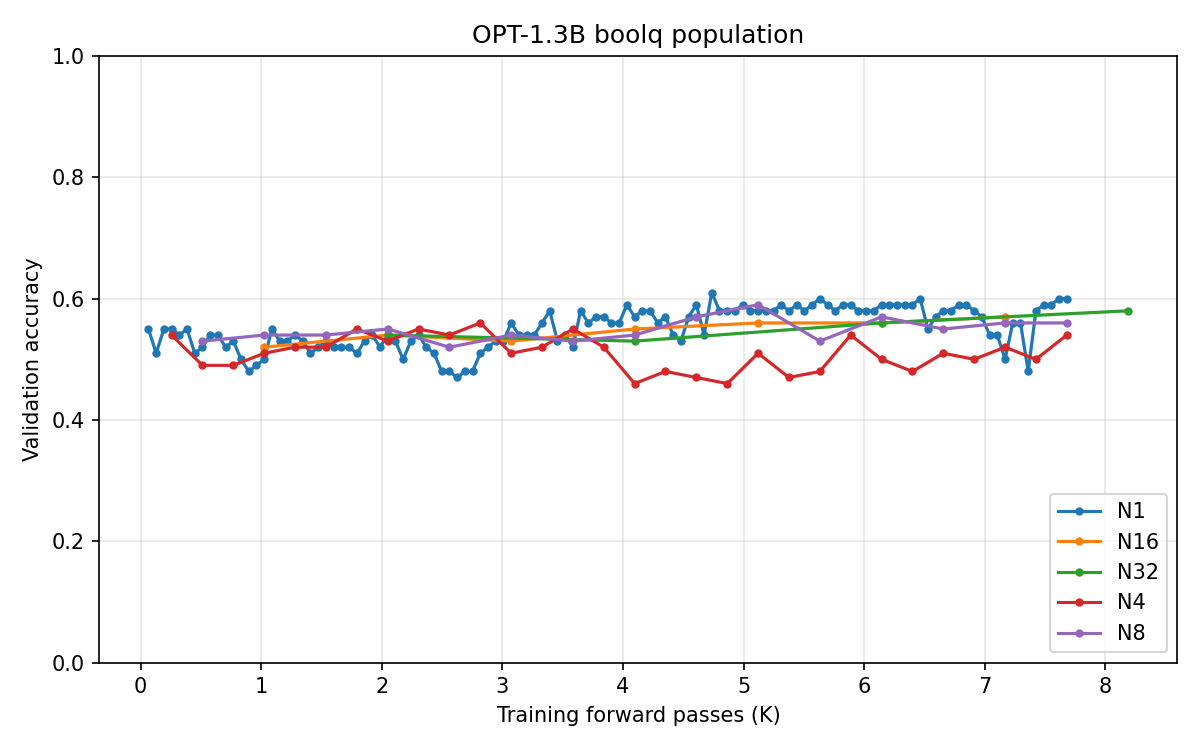
\includegraphics[width=0.7\textwidth]{empircal_plots/OPT1.3B-BoolQ.png}
  \caption{OPT-1.3B on BoolQ under binary reward across population sizes $N \in \{1, 4, 8, 16, 32\}$. All curves remain flat, indicating no learning regardless of population size. This is consistent with the high degeneracy regime ($p_0$ low, binary reward) where $\Nmin$ is not satisfied for any tested $N$.}
  \label{fig:opt13b-boolq}
\end{figure}

\subsection{Degeneracy Probe: Empirical $P(A=0)$ Measurements}

As a direct complement to the theory in Section~\ref{sec:degeneracy}, we ran the degeneracy probe (Section~\ref{sec:empirical-probe}) on \textsc{Qwen2.5-0.5B-Instruct} evaluated on GSM8K at $\sigma = 0.001$, $K = 200$ pairs, across two batch sizes:

\begin{center}
\begin{tabular}{ccccccc}
\toprule
$B$ & $p_0$ & $P(A=0)_{\text{emp}}$ & $P(A=0)_{\text{theory}}$ & Error & $\hat\rho$ & $\Nmin$ ($\delta=0.05$)\\
\midrule
16 & 0.234 & 0.215 & 0.235 & $+9\%$ & $\approx 0.40$ & 2\\
4  & 0.250 & 0.370 & 0.461 & $+25\%$ & $\approx 0.22$ & 4\\
\bottomrule
\end{tabular}
\end{center}

The theory (2$\pi$ formula, $\rho = 0.5$ assumption) overestimates $P(A=0)$ by 9--25\%. The larger error at $B=4$ is consistent with the CLT assumption requiring $B \geq 8$. The intra-pair correlation $\hat\rho$ was back-calculated from the empirical $P(A=0)$; future runs will compute $\hat\rho$ directly from stored $(R^+_k, R^-_k)$ pairs. For this model and task, $\Nmin \leq 4$ across both batch sizes --- far below the conservative bound of 29, consistent with $p_0 \approx 0.25$ being a moderately capable base model.

\subsection{Limitations}

\begin{enumerate}[leftmargin=*]
  \item As we have to run experiments where the model sizes are large and the iterations are higher, our experiments are taking substantial wall-clock time.
  \item Some experiments, such as the ES at Scale paper experiment with Qwen-2.5-Instruct on Countdown, are difficult to replicate as their setup includes multiple-GPU parallelization.
  \item Something is wrong with our current MeZO implementation as seen through the discrepancy in our SST-2 runs on OPT-13B. We initially tried to integrate MeZO logic into our repository through augmentation, but we may have to call it separately. Figure~\ref{fig:sst2-flat} shows our SST-2 run on OPT-13B remaining flat at $\approx 0.62$ across 64K forward passes despite using CE reward --- far below MeZO's reported $\approx 0.92$. This points to an implementation issue rather than a theoretical one, likely in our restricted-vocabulary CE formulation or prompt format.

\begin{figure}[h]
  \centering
  
\includegraphics[width=0.65\textwidth]{"empircal_plots/SST2 2k iters.png"}
  \caption{OPT-13B on SST-2 with CE reward (2k iterations, $\approx$64K forward passes). Validation accuracy remains flat at $\approx 0.62$, showing no learning. MeZO \citep{malladi2023mezo} reports $\approx 0.92$ on the same task and model, indicating a gap in our implementation --- likely due to restricted-vocabulary softmax versus MeZO's full-vocabulary CE loss, or prompt format mismatch.}
  \label{fig:sst2-flat}
\end{figure}
\end{enumerate}

\subsection{Next Steps}

\begin{enumerate}[leftmargin=*]
  \item Run a full experiment (20{,}000 iterations / 640{,}000 forward passes) on OPT-13B on one or two tasks to explore our hypothesis about population indifference in MeZO for cross-entropy tasks.
  \item Run population-scale experiments on Qwen-2.5-Instruct models to explore our hypothesis about the need for different population sizes for binary reward tasks.
  \item Sweep the degeneracy probe across $\sigma$ values (0.0001, 0.001, 0.01), model sizes, and tasks to characterize how $\rho$ and $P(A=0)$ vary, and to validate the general formula $P(A=0) \approx 1/\sqrt{4\pi Bp_0(1-p_0)(1-\rho)}$.
\end{enumerate}

\end{document}
